\section{Lignes}
		
	Il existe plusieurs types de lignes:
	\begin{itemize}
		\item unifilaire
		\item Bifilaire
		\item coaxiale
		\item Fibre optique
		\item A ruban
		\item \dots
	\end{itemize}
		
		elle dépende de leur géométrie, des matériaux et des conditons.
		
	\subsection{Modélisation d'une ligne}
	
		Une ligne est représenté comme  une résistance $R'$ ($\Omega/m$), une conductance $G'$, une inductance $L'$ et une capacité $C'$. Le morceau représenté si dessous se répète tous le long de la ligne
		
		\begin{figure}[htp]
			\centering
			\includegraphics[width=0.6\textwidth]{img/ModélisationLigne.png}
		\end{figure}		
		
		\begin{itemize}
			\item \textbf{$R'$} :  Résistance du matériaux (cuivre) qui transmet le signal $\rightarrow$ atténuation
			\item \textbf{L'} : Inductance champ magnétique produit par un fil et qui impacte l'autre 
			\item \textbf{$C'$} : Effet de capacité entre les 2 fils
			\item \textbf{$G'$} : Conductance très grande résistance entre les 2 fils (air ou isolant) mais courant peut tous de meme parfois passer légerement a travers
		\end{itemize}
		
		Ces parametres varient suivant le type de lignes, fréquences, matériel utilisé.
		
		L'équations des télégraphiste nous donne la relations suivantes :
		\begin{equation}
			\cfrac{\delta^2v}{\delta z^2} = LC\cfrac{\delta^2 v}{\delta t^2} + (RC + LG)\cfrac{\delta v}{\delta t} + RGv
		\end{equation}
		
		Si les pertes sont négligeables (R = G = 0)
		\begin{equation}
			\cfrac{\delta^2 v}{\delta z^2} = LC\cfrac{\delta^2 v}{\delta t^2}
		\end{equation}
		
		Elle fait le lien entre la variation de la tensions en fonction de la positions et un variation de le tension en fonction du temps
		
		
	\subsection{Effet pelliculaire}
		Effet électromagnétique qui repousse les lignes de courant  vers la surface du conducteur. les électrons vont s'amasser sur les bords
		Diminue la surface de la ligne qui est effectivement parcourie par du courant et donc augmenter la resistance de celui-ci comme $\sqrt{f}$, il est causé par la création d'un champ magnétique
		
		\begin{align*}
			\nearrow \text{fréquence} \Rightarrow \nearrow \text{effet péliculaire }\Rightarrow \nearrow \text{résistance} \Rightarrow \nearrow \text{pertes}
		\end{align*}
			
	\subsection{Atténuation}
		Peut etre calculé commet $10\log(P_{1}/P_{2})$, avec $P_1$ la puissance d'entrée, et $P_2$ la puissance de sortie. Cette atténuation se calcule en dB(décibels)
		
		On sait que $P = \cfrac{V^2}{R}$, donc, $\cfrac{P_1}{P_2} = \cfrac{v_{1}^{2}}{v_{2}^{2}}$
		
		\begin{equation}
			10\log(P_{1}/P_{2}) = 10\log\cfrac{v_{1}^{2}}{v_{2}^{2}} = 20\log\cfrac{v_{1}}{v_{2}}
		\end{equation}
		
	\subsection{Dispersion}
		La Dispersion est une sorte de distorsion du signal et donc qui impacte l'information
		
		Soit le nombre de pulsion $\omega = 2 \pi f$, le vecteur d'onde $\beta = \cfrac{2\pi}{\lambda}$, et $\lambda$ la longueur d'onde, on a la vitesse de phase (vitesse de propagation)
		\begin{equation}
			v_{ph} = \cfrac{\omega}{\beta}
		\end{equation}
		
		La dispersion d'un signal vient des différentes vitesses de déplacement des fréquences constituant une onde. L'onde a tendance a s'étaler sur le temps plus la ligne sera longue
		
	\subsection{Impédance caractéristique}
		Permet de connaitre le rapport de tension/courrant utile dans beaucoup de système pour savoir quelle tension on va récupérer en envoyant un certain courant.Impédance caractéristique désigne l'impédance en supposant que la ligne est infinie.
		
		La loi de Ohm caractérise une tension $v$ en fonction d'un résistance $r$ (ou $z$ pour resistances avec des nombres complexes) et d'un courant $i$
		\begin{equation}
			v = ri\  \text{ou} \  v = zi
		\end{equation}
		
		$z$ est totalement réel pour une résistance pure et totalement imaginaire pour une inductance/capacité pure.
		
		Dans le cas d'une ligne infinie, l'impédance d'entrée est égal a l'impédance caractéristique de la ligne $Z_{in} = Z_c$\footnote{voire slide 26 chap 2}
		
	\subsection{Exposant de propagation}
		Il arrive que il y ait de la dispersion (déphasage) et de l'affaiblissement linéique (atténuation). Soit $\alpha$ l'atténuation et $\beta$ le déphasage, on peut calculer l'exposant de propagation $\gamma$:
		\begin{equation}
			\gamma = \sqrt{(R + j \omega L)(G + j \omega C)} = \alpha + j \beta
		\end{equation}
		
		Normalement, dans une ligne, $G$ est négligeable. Deux cas se présente 
		
		\subsubsection{Cas 1}
			Dans le cas ou, $\omega L << R$, correspond au cas ou le fil a beaucoup de résistance.
			
			L'exposant de propagation en considérant $G$ et $\omega L$ nuls, car ils sont négligable au vu des hypothèses de ce cas, devient
			
			\begin{figure}[htp]
				\centering
				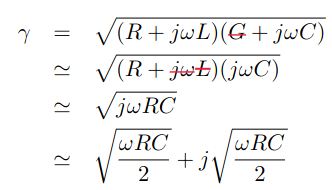
\includegraphics[width=0.4\textwidth]{img/1.png}
			\end{figure}	
			
			L'impédance caractéristique en considérant $G$ et $\omega L$ nul devient
			
			\begin{figure}[htp]
				\centering
				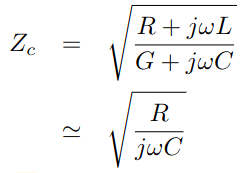
\includegraphics[width=0.3\textwidth]{img/2.png}
			\end{figure}	
				
		\subsubsection{Cas 2}
			Dans le cas ou, $\omega L >> R$, correspond au cas ou le fil a peu de résistance.
			C'est une bonne situation car peut de distorsion
			
			L'exposant de propagation en considérant $G$, car il est négligable devient:
			
			\begin{figure}[htp]
				\centering
				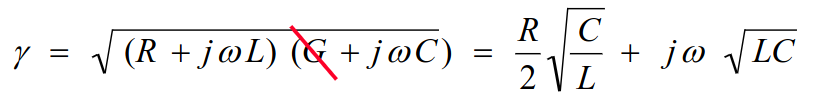
\includegraphics[width=0.6\textwidth]{img/3.png}
			\end{figure}	
			
			L'impédance caractéristique en annylant $G$ et $R$
			
			\begin{figure}[htp]
				\centering
				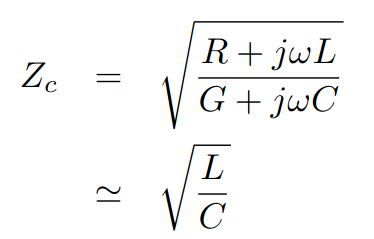
\includegraphics[width=0.2\textwidth]{img/4.png}
			\end{figure}	
			
			$\alpha$ est indépendant de $\omega$ et $\beta$ proportionnel a $\omega$. A cela s'ajoute $Z_c$ qui est réel et independant de $\omega$
			
	\newpage
			
	\subsection{Pupinisation}
	
		Le cas des anciennes lignes téléphonique basse fréquences. Plus mtn car on est a ADSL/VDSL.
		
		Pour le cas d'une ligne téléphonique $\omega L << R$, on va faire une pupinisation. C'est le fait d'insérer des inductances le long de la ligne pour augmenter artificiellement L. Avec ça, on a une réduction de l'atténuation le long de la ligne. On crée un filtre passe-bas
		
		Mais pas tres bénéfique pour une certaine bande de fréquences car elle cause l'atténuation des fréquences supérieures. vu que on a besion de ses basse fréquences, on utilise plus cette technique \footnote{Voir graph Slides 34-35 chap 2}
		
	\subsection{Lignes Bifilaire}
	
		Lignes constituée de fils parallèles séparé par un isolant, souvent rassemblé dans des quartes torsadées (quatre fils ensemble) ou encore dans une bottes de quartes (50 fils).
		
		On peut trouver de la Diaphonie (\textit{Bruit} / \textit{Crosstalk}). L'interférence d'un premier signal avec un autre (on peut par exemple entendre un autre conversation) qui passe dans une fille différente
		
		Avantage :
		\begin{itemize}
			\item Faible cout
			\item Connexion facile
			\item Pré-installation dans les bâtiments
		\end{itemize}
		
		Déavantage :
		\begin{itemize}
			\item Faible atténuation au basse fréquences
			\item Rayonnement important (probleme de confidentialité, sensibilité aux interférence)

		\end{itemize}

\begin{figure}[htp]
\centering
\begin{minipage}{.5\textwidth}
  \centering
  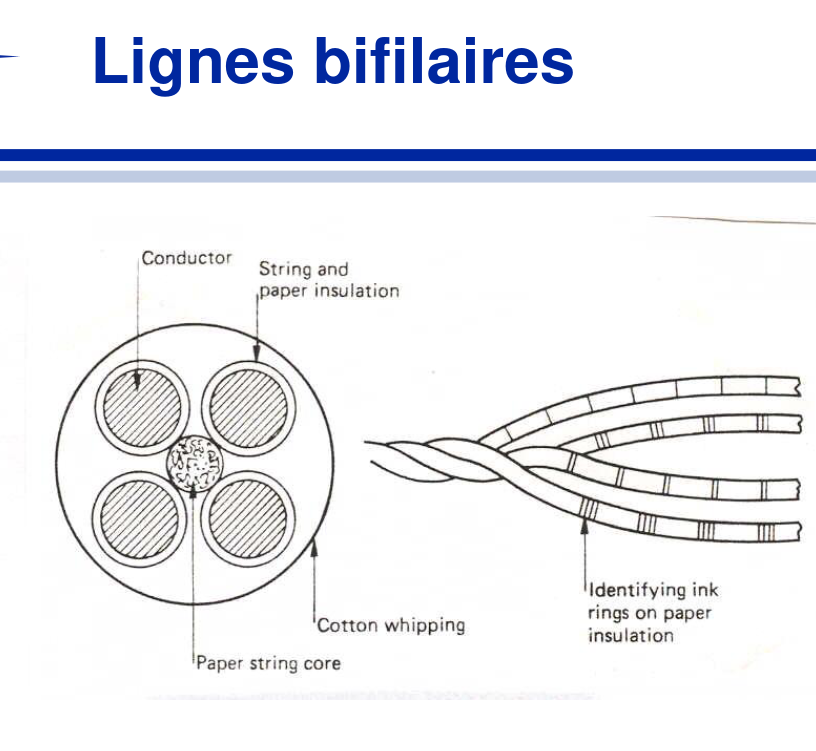
\includegraphics[width=.5\textwidth]{img/bifillaire.png}
\end{minipage}%
\begin{minipage}{.5\textwidth}
  \centering
  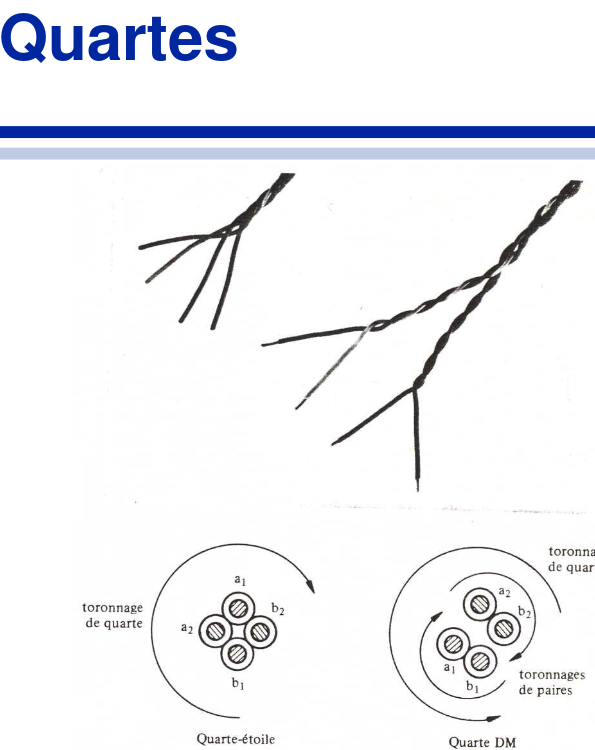
\includegraphics[width=.5\textwidth]{img/bifillaire2.png}
\end{minipage}
\begin{minipage}{.5\textwidth}
  \centering
  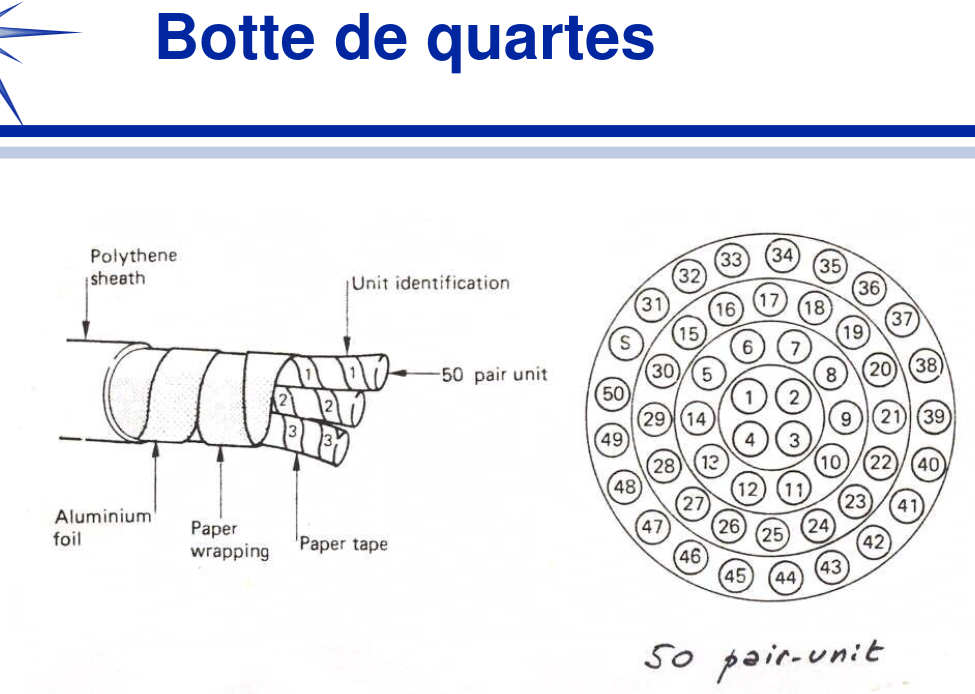
\includegraphics[width=.7\textwidth]{img/bifillaire3.png}
\end{minipage}

\end{figure}		
		
		\newpage
	\subsection{Cable coaxial}
		Câble composé d'un partie central (fil de cuivre) enveloppé d'un isolant, puis d'un blindage métallique tressée et enfin d'une gaine extérieure. Le câble est utilisé pour la transmission de la télédistribution.
		
		Avantages :
		\begin{itemize}
			\item Large bande passanet (~500 MHz)
			\item Protection contre interférence
			\item Technique éprouvée et répandue
			\item Facilité de réparation et connexion
		\end{itemize}
		
		Désavantages :
		\begin{itemize}
			\item Fréquence limité (~500 MHz)
			\item Blindage jamais parfais
		\end{itemize}
		
		\begin{figure}[htp]
\centering
\begin{minipage}{.5\textwidth}
  \centering
  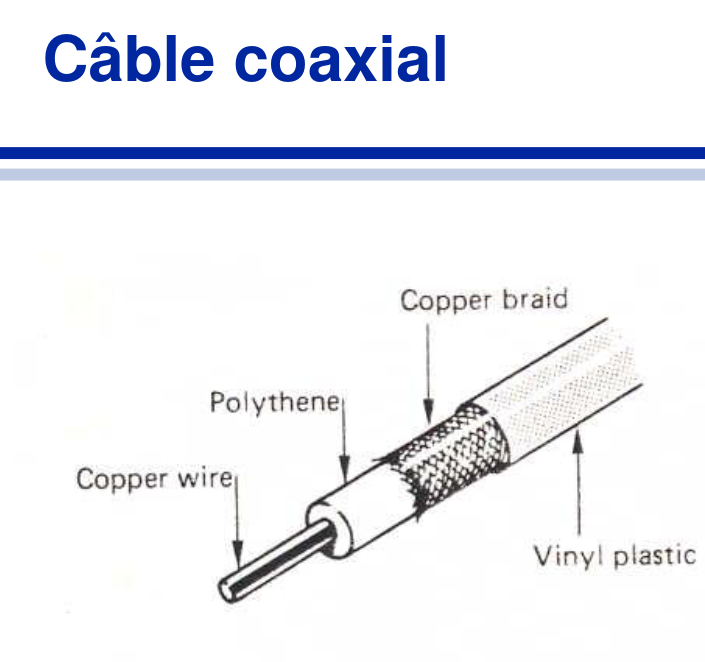
\includegraphics[width=.6\textwidth]{img/coaxial1.png}
\end{minipage}%
\begin{minipage}{.5\textwidth}
  \centering
  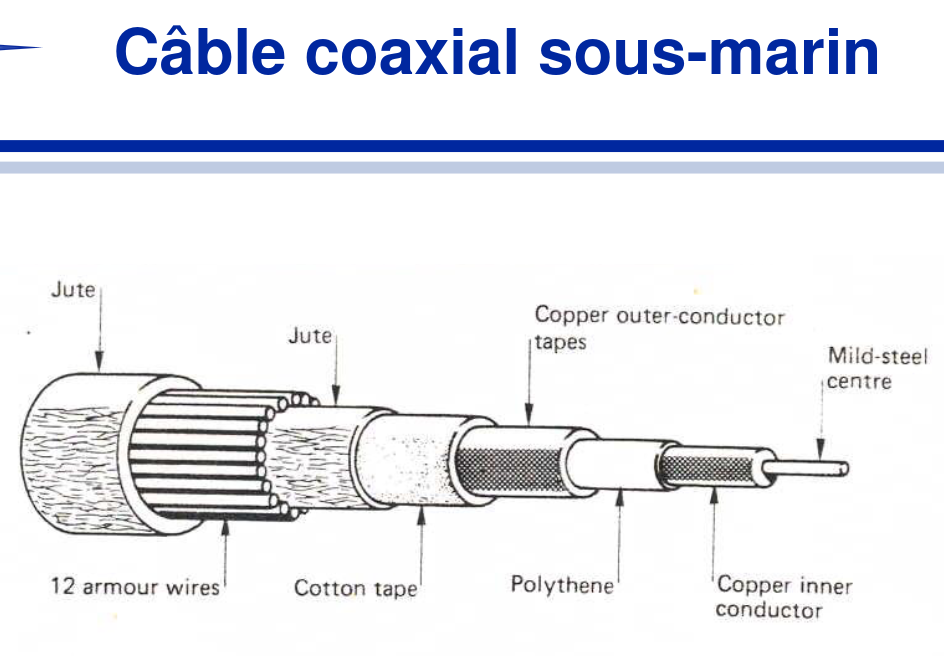
\includegraphics[width=.6\textwidth]{img/coaxial2.png}
\end{minipage}
\begin{minipage}{.5\textwidth}
  \centering
\end{minipage}

\end{figure}		

	\subsection{Fibre optique}
		C'est un conducteur de lumiere en fil en verre ou plastique trés fin qui transmet les données sous forme de lumieres
		
		Un \textbf{Mode} est un chemin emprunter par la lumiere par rapport a sa réfléxion et réfraction dans la fibre optique
		
		La \textbf{Dispertion intermodale} c'est un phénomene correspondant a l'existence de differentes vitesse possible pour la propagation des ondes. La distance parcourue par certaint modes est différentes de celle d'autre mode, il y a donc une dispersion du signal
		
		il y a plusieur moyen d'envoyer de la lumiere :
		\begin{itemize}
			\item Diode LED
			\item Diode Laser
			\item Diode Infrarouge
		\end{itemize}
		
		Avantages :
		\begin{itemize}
			\item Enorme bande passante
			\item Tres faible attenuation
			\item Immunité a l'égard des rayonnement
			\item isolation electrique
			\item Léger, fin, pas cher
		\end{itemize}
		
		Désavantages :
		\begin{itemize}
			\item Connexions difficile
			\item Réparation difficiles
			\item en développement
		\end{itemize}
		
		\subsubsection{Maniere de gerer les modes}
			\begin{enumerate}
				 \item \textbf{Fibre multimode a saut d'indice} : Les rayons réfléchissent plusieurs fois sur les parois avec un multitude d'angle different. Le saut d'indice engendre des angles tres fluctuant, il y a donc de la dispertion intermodale
				 \begin{figure}[htp]
				 	\centering
				 	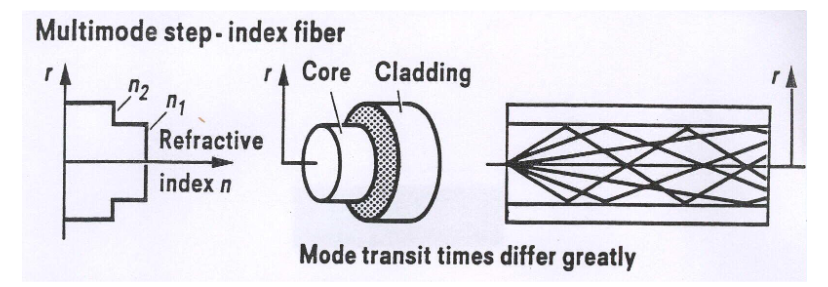
\includegraphics[width=\textwidth]{img/multimode.png}
				 \end{figure}
				 
				 \item \textbf{Fibre multimode a grandient d'indice} : On fait varier l'indice de réfraction plus l'on s'apporchera des parois afin que les différents faisceaux lumineux convergent vers le centre de la fibre. La dispersion intermodale est réduite
				 
				 \begin{figure}[htp]
				 	\centering
				 	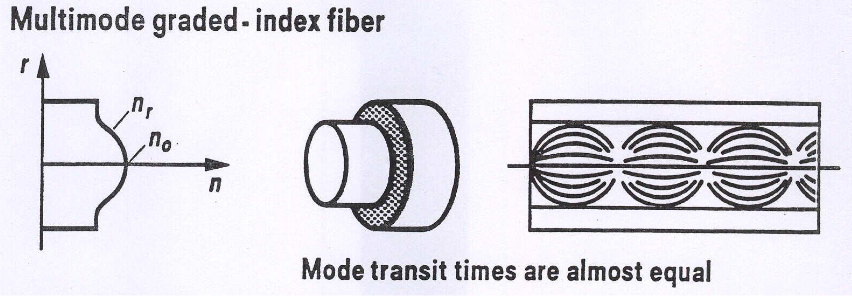
\includegraphics[width=\textwidth]{img/multimode2.png}
				 \end{figure}
				 
				 \item \textbf{Fibre Monomode} : un seul chemin au centre de la fibre. Une seul vitesse dans la fibre donc pas de dispertion intermodale.
				 
				 \begin{figure}[htp]
				 	\centering
				 	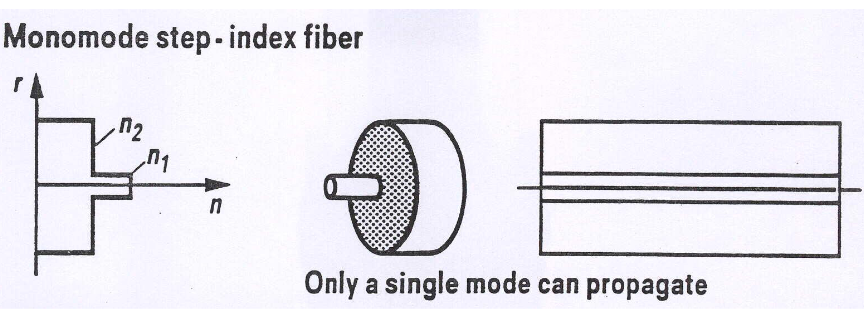
\includegraphics[width=\textwidth]{img/multimode3.png}
				 \end{figure}
			\end{enumerate}
			
			\subsubsection{Transmission dans une fibre optique}
				Un rayon rentre dans la fibre optique et est réfléchi a l'intérieur si celui-ci possède un angle adéquat qui est donc dans la range du cône d'appartenance et va parcourir la fibre optique en zigzag.
				